\section{Evaluation}
So far, we have presented a sound procedure and automated component-based framework for extracting non-functional properties of generated code. In this section, we evaluate the implementation of our approach by explaining the design of our empirical study; the research questions we set out to answer, the different methods we used to answer these questions. The experimental material is available for replication purposes at~\cite{mboussaa}.

\subsection{Research questions}
Our experiments aim at answering the following research questions:

\textbf{RQ1: Mono-objective SBSE Validation.} 
\textit{How does the proposed diversity-based exploration of optimization sequences perform compared to other mono-objective algorithms in term of memory and CPU consumption, execution time, etc.?} 
 

\textbf{RQ2: Sensitivity.} 
\textit{How sensitive are benchmark programs to compiler optimization options?}



\textbf{RQ3: Impact of optimizations on resource consumption.} 
\textit{How compiler optimizations impact on the non-functional properties of generated programs?}


\textbf{RQ4: Trade-offs between non-functional properties.} 
\textit{How can multi-objective approaches be useful to find trade-offs between non-functional properties?}

To answer these questions, we conduct several experiments using NOTICE to validate our global approach for non-functional testing of compilers using system containers.
 

\subsection{Experimental Setup}
\subsubsection{Programs used in the empirical study}
To explore the impact of compiler optimizations a set of input programs are needed. 
To do so, we use a random C program generator called Csmith~\cite{yang2011finding}.
Csmith is a tool that can generate random C programs that statically and dynamically conform to the C99 standard. It has been widely used to perform functional testing of compilers~\cite{le2014compiler,nagai2013scaling}, and not the case for checking non-functional requirements. Csmith can generate C programs that utilize a much wider range of C features including complex control flow and data structures such as pointers, arrays, and structs. Csmith programs come with their test suites that explore the structure of generated programs. 
Authors argue that Csmith is an effective bug-finding tool because it generates tests that explore atypical combinations of C language features. They argue as well, that larger programs are more effective for functional testing. Thus, we run Csmith for 24 hours and gathered the largest generated programs. We depicted 30 C programs with average source lines 12K.

Moreover, we run experiments on commonly used benchmarks in iterative compilation named Collective Benchmark (cBench)~\cite{fursin2009collective}. It is a collection of open-source sequential programs in C, targeting specific areas of the embedded market. It comes with multiple datasets assembled by the community to enable realistic benchmarking and research on program and architecture optimization. cBench contains more than 20 C programs. Selected Csmith and Cbench programs are described in more details at~\cite{mboussaa}.
\iffalse
\begin{table}[h]
	\begin{center}
		\begin{tabular}{|c|c|p{3.9cm}|}
			\hline
			\textbf{Program} & \textbf{Source lines} & \textbf{Description}\\
			\hline
			automative\_susan\_s & 1376 & Image recognition package\\
			\hline
			bzip2e & 5125 & Compress any file
			source code \\
			\hline
			bzip2d & 5125 & Decompress zipped files \\
			\hline
			office\_rsynth & 4111 & Text to speech program produced by integrating various pieces of code\\
			\hline
			consumer\_tiffmedian& 15870 & Apply the median cut algorithm to data in a TIFF file
			\\
			
			\hline
			consumer\_tiffdither& 15399 & Convert a greyscale image to bilevel using dithering
			\\
			\hline
			
		\end{tabular}
		
	\end{center}
	\caption {Description of selected benchmark programs}
\end{table}
\fi
\subsubsection{Parameter Tuning and Setting}
%Our experiments use the classical NS algorithm, where we evolve a set of optimization sequences through generations.
An important aspect for meta-heuristic search algorithms lies in the parameters tuning and selection, which is necessary to ensure not only fair comparison, but also for potential replication. 
During mono-objective search, we use to compare NS to RS and GA~\cite{cooper2002adaptive} and to NSGA-II~\cite{deb2002fast} and RS in multi-objective optimization. Each initial population/solution of different algorithms is completely random. The stopping criterion is when the maximum number of fitness evaluations is reached.
The resulting parameter values are listed in Table 3. The same parameter setting are applied to all algorithms under comparison.

NS, which is our main concern in this work, is implemented as described in Section 3. During the evolutionary process, each solution is evaluated using the novelty metric. Novelty is calculated for each solution by taking the mean of its 15 lowest dissimilar optimization sequences (considering all sequences in the current population and in the archive). Initially, the archive is empty. 
Then, to create next populations, an elite of the 10 most novel organisms is copied unchanged, after which the rest of the new population is created by tournament selection according to novelty. Standard genetic programming crossover and mutation operators are applied to these novel sequences in order to produce offspring individuals and fulfill the next population.
In the meanwhile, individuals that get a score higher than the threshold T they are automatically added to the archive as well. 
In fact, this threshold is dynamic. Every 200 evaluations, we check how many individuals have been copied into the archive. If this number is below 3, the threshold is increased by multiplying it by 0.95, whereas if solutions added to archive are above 3, the threshold is decreased by multiplying it by 1.05. 
Moreover, as the size of the archive grows, the nearest-neighbor calculations that determine the novelty scores for individuals become more computationally demanding. So to avoid having low accuracy of novelty, we choose to bound the size of the archive. Hence, it follows a first-in first-out data structure which means that when a new solution gets added, the oldest solution in the novelty archive will be discarded. Thus, we ensure individuals diversity by removing old sequences that may no longer be reachable from the current population.

The parameters of the algorithm were tuned individually in preliminary experiments. For each parameter, a set of values was tested. The parameter values chosen are the mostly used in the literature~\cite{lehman2008exploiting}. The value that yielded the highest performance scores was chosen.  

\begin{table}
	\caption{Algorithms parameters}
	\begin{tabular}{| l |l| l |l| }\hline
		\textbf{Parameter} & \textbf{Value} & \textbf{Parameter} & \textbf{Value} \\	\hhline{|=|=|=|=|}	
		Novelty nearest-k  & 15 &  Tournament size & 2\\ 
		Add archive prob. & 30 &  Mutation prob. & 0.1\\  
		Max archive size & 500 &  Crossover & 0.5  \\  
		Population size & 100 &  Nb generations &  50 \\  
		Individual length & 76 & Elitism & 10  \\ 
		Scaling archive prob. & 0.05 & Solutions added to archive & 3  \\ 	\hline
	\end{tabular}
\end{table}

\subsubsection{Evaluation Metrics Used}

For mono-objective algorithms we used to evaluate solutions using the following metrics:

-\textit{Memory Consumption Reduction (MR)}: corresponds to the percentage ratio of memory usage reduction of running container over the baseline. The baseline in our experiments is the amount of memory usage at O0 level with no optimizations. Larger values for this metric mean better performance. Memory usage is measured in bytes.

-\textit{CPU Consumption Reduction (CR)}: corresponds to the percentage ratio of CPU usage reduction over the baseline. Larger values for this metric mean better performance. The CPU consumption is measured as the CPU time in seconds.

-\textit{Speedup (S)}: corresponds to the percentage improvement in speed of execution of an optimized code compared to execution time of baseline version. Programs execution time is measured in seconds.


When comparing two mono-objective algorithms, it is usual to compare their best solutions found so far during the optimization process. However, this is not applicable when comparing two multi-objective evolutionary algorithms since each of them gives as output a set of non-dominated (Pareto equivalent) solutions. For this reason, we use performance indicator to compare multi-objective algorithms.
Thus, for multi-objective algorithms we used to evaluate solutions using the following metric:

-\textit{Hypervolume (HV)}: corresponds to the proportion of the objective space that is dominated by the Pareto front approximation returned by the algorithm and delimited by a reference point. The HV reference point is the point obtained by taking the maximum value observed. Thus, the HV metric can be computed as the area between the Pareto frontier and the HV reference point. Larger values for this metric mean better performance. The most interesting features of this indicator are its Pareto dominance compliance and its ability to capture both convergence and diversity\cite{deb2001multi}. 

\subsubsection{Setting up infrastructure}
To answer previous research questions, we configure NOTICE to run different experiments. Figure 2 shows a big picture of the testing and monitoring infrastructure considered in these experiments. 
First a meta-heuristic (mono or multi-objective) is applied to generate specific optimization sequences for the GCC compiler (step 1). During our experiments, we used GCC 4.8.4 as it is introduced in the motivation section but it is possible to choose another compiler versions using NOTICE since the process of extracting compiler optimizations is done automatically. As we are applying an evolutionary process, the new generated sequence have to be compiled and executed to gather performance metrics. We apply then the new generated optimization sequence to the input program under test (PUT) and deploy the output binary within a new instance of docker image (step 2). While executing the optimized code inside the container, performance data are sent the monitoring container (step 4) and recorded in a new times series database using our InfluxDB back-end container (step 5). Then, NOTICE accesses remotely to stored data in InfluxDB using a REST API and assigns a new performance value to the current solution(step 6). The choice of performance metric depends on experiment objectives (Memory or CPU usage, execution or compilation time, etc.).
\begin{figure}[h]
	\centering
	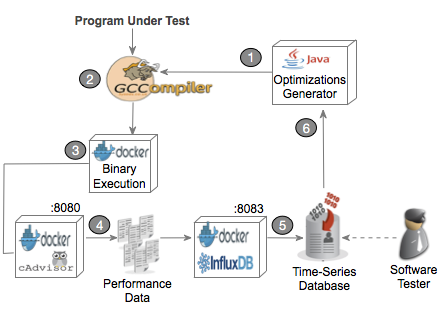
\includegraphics[width=0.9\linewidth]{Ressources/infraup.png}
	\caption{Overview of the Docker-based testing architecture}
\end{figure}







\begin{figure}[h]
	\centering
	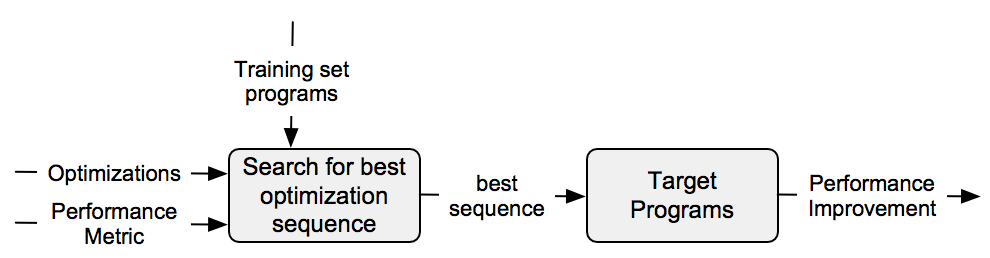
\includegraphics[width=1.\linewidth]{Ressources/sensitivity.png}
	\caption{fig}
\end{figure}

To obtain comparable and reproducible results, we use the same hardware across all experiments: an AMD A10-7700K APU Radeon(TM) R7 Graphics processor with 4 CPU cores (2.0 GHz), running Linux with a 64 bit kernel and 16 GB of system memory.


